\newpage
\subsection{Acetone + Water}

To gain better insights about the sensibility of the technique with respect
to the basis set, another test has been performed with the acetone molecule
surrounded by six water molecules. Two molecules are directly coordinated to
the carbonyl oxygen, while the remaining four coordinate the first
two molecules.

\begin{figure}[ht]
\begin{center}
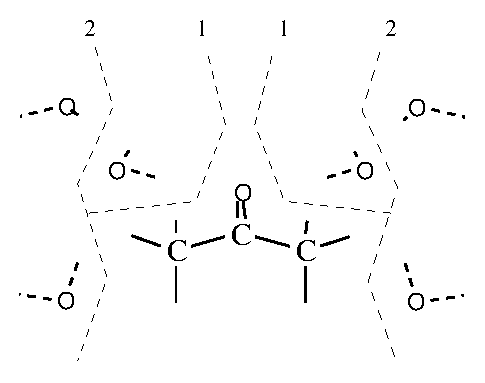
\includegraphics[width=10cm,keepaspectratio]{02_localization/images/acetone-water-frzcut-schema.eps}
\caption{\footnotesize Scheme for freeze and cut of the acetone + 6 H$_2$O
system. Surrounding water molecules have been completely frozen, and two cut
seams have been chosen to remove these molecules completely (seam ``1'') or
partially (seam ``2''). }
\label{fig:acetone-water-frzcut-schema}
\end{center}
\end{figure}

\vspace{-5mm}
The freeze and cut scheme focuses on a full freezing of the water molecules.
Two cut levels have been implemented: the first level completely removes the
water system, and the second level preserves only the two carbonyl-coordinated molecules.

The active space included five orbitals (the oxygen $n_y$ lone pair, and
carbonyl $\pi$, $\pi^{*}$, $\sigma$ and $\sigma^{*}$ orbitals) with six
active electrons. A state average optimization involving the ground state
and the $n \rightarrow \pi^{*}$ has been performed to evaluate this vertical
transition energy.

Two ANO-1 basis sets contractions have been used: the minimal set
C,O[$2s1p$], H[$1s$], hereafter called Bas-A, and an extended set
C,O[$3s2p1d$], H[$2s1p$] (Bas-B). An additional set named Bas-C is further
enriched up to C,O[$4s3p1d$], H[$2s1p$], and has been used on a smaller
system made up of the acetone molecule and two water molecules.


Tab. \ref{tbl:acetone_basis} reports the values obtained. 
The behavior of the absolute energies is as expected by previous experience:
when the cut seam is too near to the optimizable region, a difference in
absolute energy is obtained. 
\begin{center}
\begin{table}[ht]
\begin{center}
\footnotesize
\begin{tabular*}{0.80\textwidth}{l@{\hspace*{10mm}}ccc}
\hline                                                      
        &    GS       &  $n \rightarrow \pi^{*}$     &   Diff.     \\
\hline                                                      
       \multicolumn{4}{c}{Bas-A} \\
nofrz/nocut	&  -647.40071625 & -647.24175725 & 4.33 \\
frz-1/nocut &  -647.39584150 & -647.23311463 & 4.43 \\
frz-1/cut-2 &  -647.34998205 & -647.18699040 & 4.43 \\
frz-1/cut-1 &  -647.28453399 & -647.11306062 & 4.67 \\
        \multicolumn{4}{c}{Bas-B} \\
frz-1/nocut &  -648.52624523 & -648.34449917 & 4.94 \\
frz-1/cut-2 &  -645.78542705 & -645.59889274 & 5.07 \\
frz-1/cut-1 &  -644.71575515 & -644.51034075 & 5.59 \\
       \multicolumn{4}{c}{Bas-B non-ortho}  \\
frz-1/cut-2 &  -648.70019443 & -648.52408727 & 4.79 \\
frz-1/cut-1 &  -648.93490599 & -648.73207516 & 5.52 \\
\hline
\end{tabular*}
\end{center}
\caption{\footnotesize CAS+S absolute energies (Hartree) and energy
difference (eV) between ground state and $n \rightarrow \pi^{*}$ state of
acetone + 6 H$_2$O, using the minimal Bas-A basis set and the extended basis
set Bas-B (see text). Bas-B non-ortho refers to an evaluation with 
non-orthonormal orbitals.}
\label{tbl:acetone_basis}
\end{table}
\end{center}


The relative behavior, however, is poorly
affected.  When a large basis set is used, the absolute energy drift is
strongly increased. The larger Bas-B basis set produces a very steep
variation compared to the minimal Bas-A. 

\begin{figure}[ht]
\begin{center}
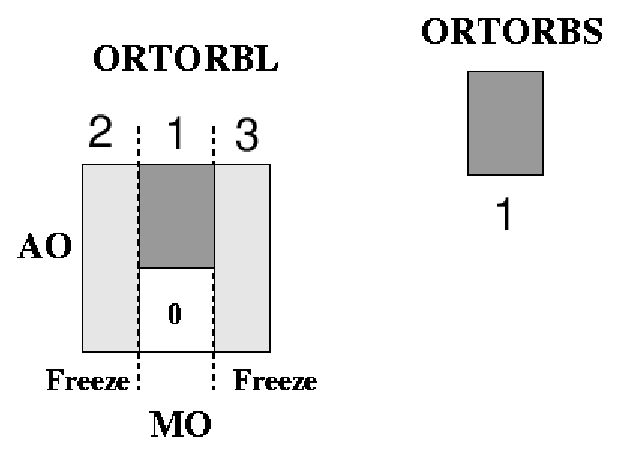
\includegraphics[width=7cm,keepaspectratio]{02_localization/images/matrix-2.eps}
\caption{\footnotesize A visual representation of the hierarchical
orthonormalization performed on the orbitals. The non-frozen orbitals
(marked with ``1'' in figure) are orthonormalized among themselves.
Then, frozen core orbitals (marked with ``2'' in figure) are orthonormalized
among themselves and against the non-frozen ones. Finally, the frozen
virtual orbitals (marked with ``3'') are orthonormalized against ``1'' and ``2''.
}
\label{fig:matrix-2}
\end{center}
\end{figure}



An additional effect must be considered responsible of the reported
behavior.  Further investigations, performed with the smaller system acetone
+ 2 H$_2$O, revealed a problem related to the molecular orbital hierarchical
orthonormalization (Fig.~\ref{fig:matrix-2}). After the cut action,
orbitals are no longer orthonormal, and the orthonormalization procedure
aims at restoring this orthonormality. 

The first class of orbitals performing the orthonormalization is the
non-frozen zone (marked ``1'' in Fig.~\ref{fig:matrix-2}) which remains
described in the smaller AO space. This class must be treated first, in
order to preserve itself inside this restricted space.

The second class is the frozen core orbitals class (marked ``2'' in
Fig.~\ref{fig:matrix-2}). When this class is orthonormalized with respect to
the first one, orthonormalization tails are produced, effectively changing
the core orbitals. The weight and spatial distribution of these tails is
bound to the atomic basis set used to describe the molecular system,
therefore larger basis sets produce stronger effects.

This situation is different from the previously reported phenomenon in
7Z-13 ammoniotridec-7-enoate in the frz-3/cut-3 analysis, where hydrogen
atoms were removed from non-frozen orbitals. In the current case, frozen
orbitals are modified due to orthonormality needs, which impose tails toward
nearby atoms. These tails introduce an artificial charge shift toward these
atoms, and in particular those involved in the physical process under
study, resulting in convergence problems or a high energy drift. The process
sometimes makes impossible for the evaluation to converge.

Molden plots have been performed on the smaller system with only two water
molecules. The contour factor is 0.03. Fig.~\ref{fig:acetone_tails} shows a
clear difference between the water OH bond with the Bas-C contraction and
the Bas-A contraction.

\begin{figure}[ht]
\begin{center}
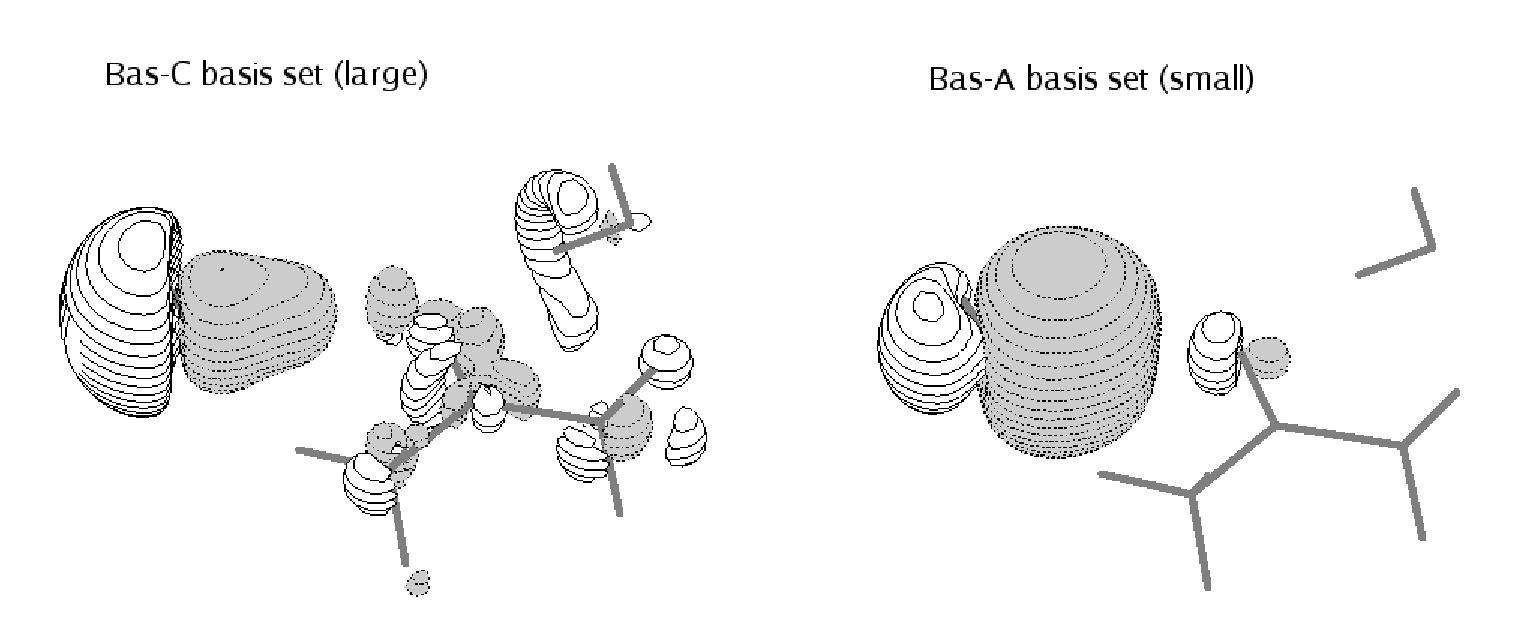
\includegraphics[width=12cm,keepaspectratio]{02_localization/images/acetone_tails.eps}
\caption{\footnotesize The water OH bond on the small acetone +
2H$_2$O system, using the large basis set Bas-C and the small Bas-A. The
difference in spatial distribution of the orthonormalization tails is
clearly visible. }
\label{fig:acetone_tails}
\end{center}
\end{figure}

\vspace{-5mm}
The nature of this problem is independent of the frozen spacer between the
removed zone and the non-frozen zone, but related to the frozen/non-frozen
seam. The problem do not arise when cut is not performed, and consequently
the resulting orbitals do not incur in orthonormalization. 

At first glance, a possible solution is to keep the frozen/non-frozen seam
as much far as possible from the region interested in the chemical
phenomenon, leading to absolute energy drifts but prevent tails to
act on the active space. However, this goes in the direction of incrementing
the computational cost of the final evaluation, enlarging the non-frozen
zone in a large basis regime.

Another possible solution has been attempted working with a non-orthonormal
basis set. Frozen orbitals are not orthonormalized with respect to the
non-frozen ones, and the results obtained (Tab.~\ref{tbl:acetone_basis}
non-ortho) show a cleaner behavior. However, it must be pointed out that this
procedure is not strictly formal under the assumptions made for the current
theoretical deployment, and the convergence is very slow. An improvement in
the theoretical asset is needed to formally work around this problem.
